
\setlength{\tabcolsep}{8pt}
% [ Check RGB-D single modality ]
\begin{table}[t]
\begin{center}
\vspace{3mm}
\caption{Top-1 \textit{mean} accuracy ($\%$) of different common-use architectures, over all $D_i \rightarrow D_j$ combinations on both seen and unseen test sets in \textit{offline-trimmed} setting. }
\label{tab:backbone}
\begin{tabular}{lccccc}%{lC{1.5cm}C{1.5cm}C{1.5cm}}
\toprule\noalign{\smallskip}
\multicolumn{5}{c}{\normalsize\textsc{EPIC-Kitchens 55}} \\
\noalign{\smallskip}
\cline{1-5}
\noalign{\smallskip}
Network  & Sampling & Params & Seen & Unseen \\
\noalign{\smallskip}
\toprule\noalign{\smallskip}
\multirow{1}{*}{\centering TSN} 
  & U 5x5 & 10.7M & 60.88 & 31.55 \\
 
  \noalign{\smallskip}

 \multirow{1}{*}{\centering TSN-TRN} 
  & U 5x5  & 18.3M & 63.13 & 32.42 \\
 

 \noalign{\smallskip}
\multirow{1}{*}{\centering TSM} 
  & U 5x5 &  24.3M & \textbf{71.48} & 35.97 \\
 
  
   \noalign{\smallskip}
\multirow{1}{*}{\centering TSM-TRN} 
  & U 5x5 & - & 69.52 & 36.05 \\
 
  \hline 
 \noalign{\smallskip}
\multirow{1}{*}{\centering I3D }
  & U 16x5 & 12.4M & 67.34 & \textbf{43.89} \\ 
 
 \noalign{\smallskip}
\multirow{1}{*}{\centering I3D }
  & D 16x5 & 12.4M & 67.08 & 42.42 \\
    \hline
 \noalign{\smallskip}
\multirow{1}{*}{\centering X3D-XS }
  & U 5x5 & 3.8M & 51.46 & 36.39 \\ 	

 \noalign{\smallskip}
\multirow{1}{*}{\centering X3D-XS }
  & D 16x5 & 3.8M & 48.45 & 32.66 \\
  

    \noalign{\smallskip}
\multirow{1}{*}{\centering MoViNet-A0 }
  & U 5x5 & 3.1M & \rev{62.17} & \rev{39.25} \\

  
     \noalign{\smallskip}
\multirow{1}{*}{\centering MoViNet-A0 }
  & D 16x5 & 3.1M & \rev{64.17} & \rev{40.68} \\

\bottomrule
\end{tabular}
\end{center}
\vspace{-5mm}
\end{table}
\setlength{\tabcolsep}{1.4pt}



\setlength{\tabcolsep}{7pt}
% [ Check RGB-D single modality ]
\begin{table}[t]
\begin{center}
\vspace{3mm}
\caption{Top-1 \textit{mean} accuracy ($\%$), over all $D_i \rightarrow D_j$ combinations on both seen and unseen test sets in both \textit{offline-trimmed} setting and \textit{streaming-trimmed} setting}
\label{tab:offlinevsstream}
\begin{tabular}{lccccc}%{lC{1.5cm}C{1.5cm}C{1.5cm}}
\toprule\noalign{\smallskip}
\multicolumn{5}{c}{\normalsize\textsc{EPIC-Kitchens 55}} \\
\noalign{\smallskip}
\cline{1-5}
\noalign{\smallskip}
Network & Mode & Sampling & Seen & Unseen \\

  \hline
 \noalign{\smallskip}
\multirow{1}{*}{\centering I3D  }
 & Offline  & D 16x5 & 67.08 & 42.42 \\
 
 
 \noalign{\smallskip}
\multirow{1}{*}{\centering X3D-XS  }
 & Offline  & D 16x5 & 48.45 & 32.66 \\


 \noalign{\smallskip}
\multirow{1}{*}{\centering MoViNet-A0  }
 & Offline  & D 16x5 & \rev{64.17} & \rev{40.68} \\

\hline

 \noalign{\smallskip}
\multirow{1}{*}{\centering I3D  }
 & Streaming & All Stream & \textbf{63.38} & \textbf{40.57} \\
 

 \noalign{\smallskip}
\multirow{1}{*}{\centering X3D-XS  }
 & Streaming & All Stream & 43.37 & 32.31 \\
 	
  
 \noalign{\smallskip}
\multirow{1}{*}{\centering MoViNet-A0  }
 & Streaming & All Stream & 62.24 & 39.59 \\

\bottomrule
\end{tabular}
\end{center}
\vspace{-5.5mm}
\end{table}

\setlength{\tabcolsep}{1.4pt}


\begin{figure}[t!]
\vspace{2mm}
\centering
\hspace{-15px}
\begin{minipage}[t]{\columnwidth}
 %   \subfloat[]{
     \resizebox {\columnwidth} {!} {
        \begin{tikzpicture}
        \pgfplotsset{every axis legend/.append style={
at={(0.5,1.03)},
anchor=south}}

        % LEFT AXIS
        % =========
        \begin{axis}[
          enlargelimits=false,
          ylabel={Top-1 Accuracy (\%)},
          xlabel={Percentage (\%)},
           xmin=0, xmax=100,
           ymin=26, ymax=68,
          xtick={0,20,40,60,80,100},
          ytick={30,40,50,60},
          %legend pos=south west,
          xmajorgrids=true,
          ymajorgrids=true,
          grid style=dashed,
          width=15cm,
          height=8cm,
          legend columns=3,
          legend style={font=\LARGE},
          label style={font=\LARGE},
          tick label style={font=\LARGE},
        legend style={draw=none},
        every axis plot/.append style={ultra thick},
        every mark/.append style={mark size=50pt}
        ]
        
        \addplot[
          color=MaterialBlue800]
        table[x index=0,y index=1,col sep=comma]
        {tex/Tables/Tab/I3D_full_sup.txt};
               \addlegendentry{I3D-(seen)} 
               
               
       \addplot[
          color=MaterialOrange800]
        table[x index=0,y index=1,col sep=comma]
        {tex/Tables/Tab/movinet_sup.txt};
               \addlegendentry{MoViNet-(seen)} 
               
        \addplot[
          color=greeno]
        table[x index=0,y index=1,col sep=comma]
        {tex/Tables/Tab/X3D_sup.txt};
               \addlegendentry{X3D-(seen)} 

         
       % \addlegendentry{Single-DG-RNA} 
        
        
        % An \addplot for each line
        \addplot[
          color=MaterialBlue800, dashed]
        table[x index=0,y index=1,col sep=comma]
        {tex/Tables/Tab/I3D_full_cross.txt};
       \addlegendentry{I3D-(unseen)} 


         
       % \addlegendentry{Single-DG-RNA} 
        
        
        % An \addplot for each line
        \addplot[
          color=MaterialOrange800, dashed]
        table[x index=0,y index=1,col sep=comma]
        {tex/Tables/Tab/movinet_cross.txt};
       \addlegendentry{MoViNet-(unseen)}
      
         
       % \addlegendentry{Single-DG-RNA} 
        
        
        % An \addplot for each line
        \addplot[
          color=greeno, dashed]
        table[x index=0,y index=1,col sep=comma]
        {tex/Tables/Tab/X3D_cross.txt};
       \addlegendentry{X3D-(unseen)} 

        \end{axis}
        
        \end{tikzpicture}%
      }

    \end{minipage}

\caption{MoViNet, X3D and I3D performance with respect to the percentage of video observed}
\vspace{-0.4cm}
\label{fig:videoperc}
\end{figure}

\section{Experiments}
%
\begin{figure}[t!]
\centering
\begin{minipage}[t]{0.44\textwidth}
 %   \subfloat[]{
     \resizebox {\columnwidth} {!} {
        \begin{tikzpicture}
        \pgfplotsset{every axis legend/.append style={
at={(0.5,1.03)},
anchor=south}}

        % LEFT AXIS
        % =========
        \begin{axis}[
          enlargelimits=false,
          ylabel={\large  Seen Acc. (\%)},
          xlabel={},
           xmin=0, xmax=72,
           ymin=22, ymax=53,
          xtick={0,8,16,32,48,64},
          ytick={20,25,30,35,40,45,50},
          %legend pos=south west,
          ymajorgrids=true,
          grid style=dashed,
          width=10cm,
          height=4.5cm,
          legend columns=2,
        legend style={draw=none},
        every axis plot/.append style={ultra thick},
        every mark/.append style={mark size=50pt}
        ]
        
        \addplot[
          color=MaterialBlue800,
          mark=square*]
        table[x index=0,y index=1,col sep=comma]
        {tex/Tables/Tab/seen-clean-static-i3d.txt};
               \addlegendentry{I3D-(with clean)} 
         
        
        
        % An \addplot for each line
        \addplot[
          color=MaterialOrange800,
          mark=oplus*]
        table[x index=0,y index=1,col sep=comma]
        {tex/Tables/Tab/seen-clean-static-MoViNet.txt};
       \addlegendentry{MoViNet-(with clean)} 
       
       %%%%%%%%%%%%%%%%%%%%
       %  no clean buffer %
       %%%%%%%%%%%%%%%%%%%%
       
        \addplot[dotted,
          color=MaterialBlue800,]
        table[x index=0,y index=1,col sep=comma]
        {tex/Tables/Tab/seen-noclean-i3d.txt};
               \addlegendentry{I3D-(w/o clean)} 
         
        
        
        % An \addplot for each line
        \addplot[dotted,
          color=MaterialOrange800,]
        table[x index=0,y index=1,col sep=comma]
        {tex/Tables/Tab/seen-noclean-MoViNet.txt};
       \addlegendentry{MoViNet-(w/o clean)} 


        \end{axis}
        
        \end{tikzpicture}%
      }

    \end{minipage}
\begin{minipage}[t]{0.44\textwidth}
 %   \subfloat[]{
     \resizebox {\columnwidth} {!} {
        \begin{tikzpicture}
        \pgfplotsset{every axis legend/.append style={
at={(0.5,1.03)},
anchor=south}}

        % LEFT AXIS
        % =========
        \begin{axis}[
          enlargelimits=false,
          ylabel={\large Unseen Acc. (\%)},
          xlabel={},
           xmin=0, xmax=72,
           ymin=20, ymax=37,
          xtick={0,8,16,32,48,64},
          ytick={22,24,28,30,32,34},
          %legend pos=south west,
          ymajorgrids=true,
          grid style=dashed,
          width=10cm,
          height=4.5cm,
          legend columns=2,
        legend style={draw=none},
        every axis plot/.append style={ultra thick},
        every mark/.append style={mark size=50pt}
        ]
        
        \addplot[
          color=MaterialBlue800,
          mark=square*]
        table[x index=0,y index=1,col sep=comma]
        {tex/Tables/Tab/unseen-clean-static-i3d.txt};
               \addlegendentry{I3D-(with clean)} 

         
       % \addlegendentry{Single-DG-RNA} 
        
        
        % An \addplot for each line
        \addplot[
          color=MaterialOrange800,
          mark=oplus*]
        table[x index=0,y index=1,col sep=comma]
        {tex/Tables/Tab/unseen-clean-static-MoViNet.txt};
       \addlegendentry{MoViNet-(with clean)} 
        
        
       %%%%%%%%%%%%%%%%%%%%
       %  no clean buffer %
       %%%%%%%%%%%%%%%%%%%%
       
        \addplot[dotted,
          color=MaterialBlue800,]
        table[x index=0,y index=1,col sep=comma]
        {tex/Tables/Tab/unseen-noclean-i3d.txt};
               \addlegendentry{I3D-(w/o clean)} 
         
        
        
        % An \addplot for each line
        \addplot[dotted,
          color=MaterialOrange800,]
        table[x index=0,y index=1,col sep=comma]
        {tex/Tables/Tab/unseen-noclean-MoViNet.txt};
       \addlegendentry{MoViNet-(w/o clean)} 
        
        \end{axis}  
        
        \end{tikzpicture}%
      }

    \end{minipage}
%%%%%%%%%%%%%
%   graph   %
%%%%%%%%%%%%%

%\begin{minipage}[t]{0.44\textwidth}
 %   \subfloat[]{
%    \resizebox {\columnwidth} {!}{
%    \centering
%    %%%%%%%%%%%%%%%%%%%%%%%%%%%%%%%%%%%%%%%%%%%%%%%%%%%%%%%%%%%%%%%
%
% Welcome to Overleaf --- just edit your LaTeX on the left,
% and we'll compile it for you on the right. If you open the
% 'Share' menu, you can invite other users to edit at the same
% time. See www.overleaf.com/learn for more info. Enjoy!
%
%%%%%%%%%%%%%%%%%%%%%%%%%%%%%%%%%%%%%%%%%%%%%%%%%%%%%%%%%%%%%%%
%\usepgfplotslibrary{external}
%\tikzexternalize

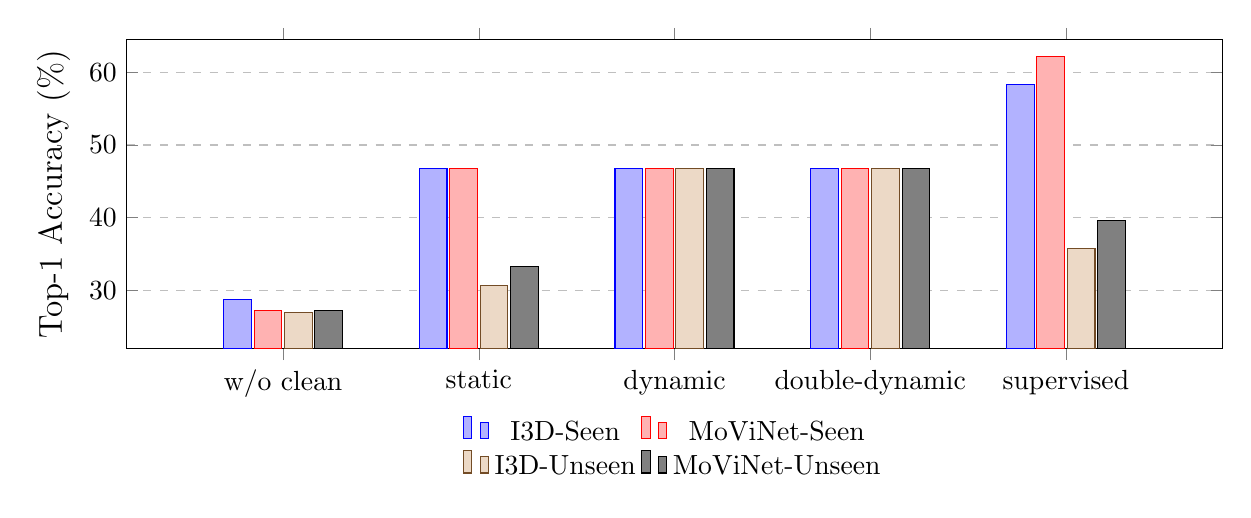
\begin{tikzpicture}
\centering
\begin{axis}[
symbolic x coords={w/o clean, static, dynamic, double-dynamic, supervised},
	ylabel=\large Top-1 Accuracy (\%),
	enlargelimits=false,
	ybar=1pt, enlarge x limits=0.2,
	xtick=data,
	ymin=22.0,
    ymax=64.5,
    ymajorgrids=true,
    legend style={draw=none},
          grid style=dashed,
          width=15.5cm,
          height=5.5cm,
         legend style={at={(0.5,-0.2)},
	    anchor=north,legend columns=2}, 
        every axis plot/.append 
        every mark/.append style={mark size=52pt}
]
\addplot 
	coordinates {(w/o clean,28.73) (static,46.77) (dynamic,46.77) (double-dynamic,46.77)
	(supervised,58.33) };
	\addlegendentry{I3D-Seen} 
\addplot 
	coordinates {(w/o clean,27.20) (static,46.71) (dynamic,46.71)(double-dynamic,46.77)
	(supervised,62.24) };
	\addlegendentry{MoViNet-Seen} 
\addplot 
	coordinates {(w/o clean,26.96) (static,30.71) (dynamic,46.71)(double-dynamic,46.77)
	(supervised,35.71) };
\addlegendentry{I3D-Unseen} 
\addplot 
	coordinates {(w/o clean,27.20) (static,33.30) (dynamic,46.71)(double-dynamic,46.77)
	(supervised,39.59) };
\addlegendentry{MoViNet-Unseen} 

\end{axis}
\end{tikzpicture}



%    }
%    \vspace{0.4cm}
%    \end{minipage}    


%%%%%%%%%%%%%%
%   graph 2  %
%%%%%%%%%%%%%%
%\begin{minipage}[t]{0.44\textwidth}
% %   \subfloat[]{
%    \resizebox {\columnwidth} {!}{
%    \centering
%    %%%%%%%%%%%%%%%%%%%%%%%%%%%%%%%%%%%%%%%%%%%%%%%%%%%%%%%%%%%%%%%
%
% Welcome to Overleaf --- just edit your LaTeX on the left,
% and we'll compile it for you on the right. If you open the
% 'Share' menu, you can invite other users to edit at the same
% time. See www.overleaf.com/learn for more info. Enjoy!
%
%%%%%%%%%%%%%%%%%%%%%%%%%%%%%%%%%%%%%%%%%%%%%%%%%%%%%%%%%%%%%%%
%\usepgfplotslibrary{external}
%\tikzexternalize

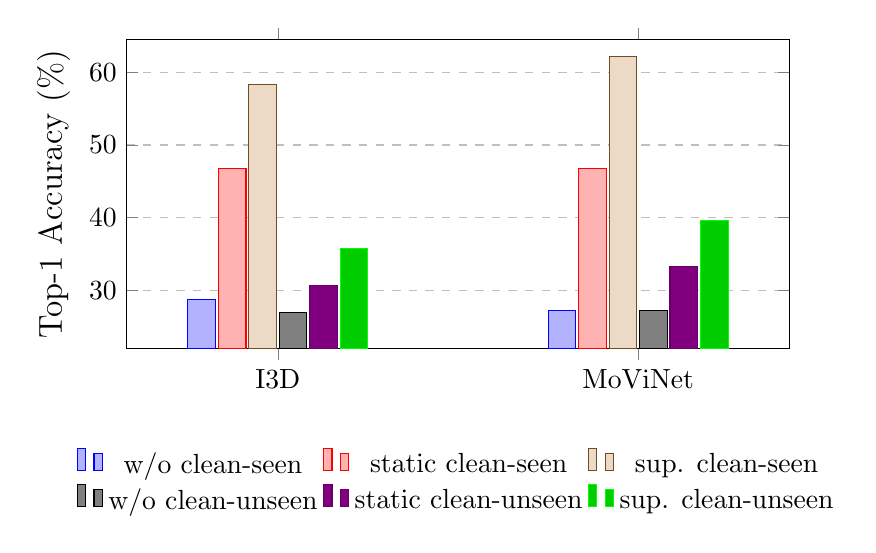
\begin{tikzpicture}
\begin{axis}[
symbolic x coords={I3D, MoViNet},
	ylabel=\large Top-1 Accuracy (\%),
	enlargelimits=false,
	ybar=1pt, enlarge x limits=0.42,
	xtick=data,
	ymin=22.0,
    ymax=64.5,
    ymajorgrids=true,
    legend style={draw=none},
          grid style=dashed,
          width=10cm,
          height=5.5cm,
         legend style={at={(0.5,-0.3)},
	    anchor=north,legend columns=3}, 
        every axis plot/.append 
        every mark/.append style={mark size=52pt}
]
\addplot 
	coordinates {
	            (I3D,28.73)
	            (MoViNet,27.20)
	};
	\addlegendentry{w/o clean-seen} 
\addplot 
	coordinates {
	            (I3D,46.77)
	            (MoViNet,46.71)
	};
	\addlegendentry{static clean-seen} 
\addplot 
	coordinates {
	            (I3D,58.33)
	            (MoViNet,62.24)
	};
	\addlegendentry{sup. clean-seen} 
	
	
	

\addplot 
	coordinates {
	            (I3D,26.96)
	            (MoViNet,27.20)
	};
	\addlegendentry{w/o clean-unseen} 

\addplot 
	coordinates {
	            (I3D,30.71)
	            (MoViNet,33.30)
	};
	\addlegendentry{static clean-unseen} 

\addplot 
	coordinates {
	            (I3D,35.71)
	            (MoViNet,39.59)
	};
	\addlegendentry{sup. clean-unseen} 

\end{axis}
\end{tikzpicture}



%    }
%    
%    \end{minipage}    
        
    

\caption{\textbf{Static boundary localization.} Top-1 \textit{mean} accuracy ($\%$), over all $D_i \rightarrow D_j$ combinations on both seen (up) and unseen (down) test sets in \textit{online-trimmed} setting, with different clean buffer strategy w.r.t the no-clean buffer. }
\label{fig:clean_static}
\end{figure}
%
\begin{figure}[t!]
\centering
\begin{minipage}[t]{0.44\textwidth}
 %   \subfloat[]{
     \resizebox {\columnwidth} {!} {
        \begin{tikzpicture}
        \pgfplotsset{every axis legend/.append style={
at={(0.5,1.03)},
anchor=south}}


        % LEFT AXIS
        % =========
        \begin{axis}[
          enlargelimits=false,
          ylabel={\large Seen Acc. (\%)},
          xlabel={},
           ymin=38.5, ymax=56,
           xmin=0.2, xmax=1.1,
          xtick={0.3,0.4,0.5,0.6,1},
          ytick={40,42,45,50,53},
          %legend pos=south west,
          ymajorgrids=true,
          grid style=dashed,
          width=10cm,
          height=4.5cm,
          legend columns=2,
        legend style={draw=none},
        every axis plot/.append style={ultra thick},
        every mark/.append style={mark size=50pt}
        ]
        
        \addplot[
          color=MaterialBlue800,
          mark=square*]
        table[x index=0,y index=1,col sep=comma]
        {tex/Tables/Tab/seen-clean-dynamically-i3d.txt};
               \addlegendentry{I3D dynamic} 

         
       % \addlegendentry{Single-DG-RNA} 
        
        
        % An \addplot for each line
        \addplot[
          color=MaterialOrange800,
          mark=oplus*]
        table[x index=0,y index=1,col sep=comma]
        {tex/Tables/Tab/seen-clean-dynamically-MoViNet.txt};
       \addlegendentry{MoViNet dynamic} 
        
    \addplot[dotted,
          color=MaterialBlue800,
          mark=triangle]
        table[x index=0,y index=1,col sep=comma]
        {tex/Tables/Tab/clean-statically-i3d-seen.txt};
       \addlegendentry{I3D static} 
      
      \addplot[dotted,
          color=MaterialOrange800,
          mark=triangle]
        table[x index=0,y index=1,col sep=comma]
        {tex/Tables/Tab/clean-statically-MoViNet-seen.txt};
       \addlegendentry{MoViNet static} 
    
        
        
        \end{axis}
        
        \end{tikzpicture}%
      }

    \end{minipage}

\begin{minipage}[t]{0.44\textwidth}
 %   \subfloat[]{
    \vspace{0.4cm}
     \resizebox {\columnwidth} {!} {
        \begin{tikzpicture}
        \pgfplotsset{every axis legend/.append style={
at={(0.5,1.03)},
anchor=south}}

        % LEFT AXIS
        % =========
        \begin{axis}[
          enlargelimits=false,
          ylabel={\large Unseen Acc. (\%)},
          xlabel={},
           xmin=0.2, xmax=1.1,
           ymin=28, ymax=37,
          xtick={0.3,0.4,0.5,0.6,1},
          ytick={22,24,28,30,32,34,36},
          %legend pos=south west,
          ymajorgrids=true,
          grid style=dashed,
          width=10cm,
          height=4.5cm,
          legend columns=2,
        legend style={draw=none},
        every axis plot/.append style={ultra thick},
        every mark/.append style={mark size=50pt}
        ]
        
        \addplot[
          color=MaterialBlue800,
          mark=square*]
        table[x index=0,y index=1,col sep=comma]
        {tex/Tables/Tab/unseen-clean-dynamically-i3d.txt};
        \addlegendentry{I3D dynamic} 

         
       % \addlegendentry{Single-DG-RNA} 
        
        
        % An \addplot for each line
        \addplot[
          color=MaterialOrange800,
          mark=oplus*]
        table[x index=0,y index=1,col sep=comma]
        {tex/Tables/Tab/unseen-clean-dynamically-MoViNet.txt};
       \addlegendentry{MoViNet dynamic} 
       
       \addplot[dotted,
          color=MaterialBlue800,
          mark=triangle]
        table[x index=0,y index=1,col sep=comma]
        {tex/Tables/Tab/clean-statically-i3d-unseen.txt};
       \addlegendentry{I3D static} 
      
      \addplot[dotted,
          color=MaterialOrange800,
          mark=triangle]
        table[x inde x=0,y index=1,col sep=comma]
        {tex/Tables/Tab/clean-statically-MoViNet-unseen.txt};
       \addlegendentry{MoViNet static} 
       
       
       
       
        \end{axis}

        \end{tikzpicture}%
      }

    \end{minipage}
    
\caption{\textbf{Dynamic boundary localization.} Top-1 \textit{mean} accuracy ($\%$), over all $D_i \rightarrow D_j$ combinations on both seen (up) and unseen (down) test sets in \textit{online-trimmed} setting, with different threshold-values. }
\label{fig:dynamically_clean}
\end{figure}
%
\begin{figure*}[t!]
\centering
%\addlegendentry{I3D-(SBL)} 
%\addlegendentry{MoViNet-(SBL)} 
%\addlegendentry{I3D-(w/o SBL)} 
%\addlegendentry{MoViNet-(w/o SBL)}
\hspace{-10px}
\begin{minipage}[t]{0.255\textwidth}
 %   \subfloat[]{
     \resizebox {\columnwidth} {!} {
        \begin{tikzpicture}
        \pgfplotsset{every axis legend/.append style={
at={(0.41,1.03)},
anchor=south}}
        % LEFT AXIS
        % =========
        \begin{axis}[
          enlargelimits=false,
          ylabel={Seen Acc. (\%)},
          xlabel={},
           xmin=4, xmax=68,
           ymin=22, ymax=65,
          xtick={0,8,16,32,48,64},
          ytick={20,25,30,35,40,45,50,55,60},
          %legend pos=south west,
          ymajorgrids=true,
          grid style=dashed,
          width=6.7cm,
          height=6.25cm,
          legend columns=2,
        legend style={draw=none},
        every axis plot/.append style={ultra thick},
        every mark/.append style={mark size=50pt}
        ]
        \addplot[
          color=MaterialBlue800,
          mark=square*]
        table[x index=0,y index=1,col sep=comma]
        {tex/Tables/Tab/seen-clean-static-i3d.txt};
        \addlegendentry{I3D-(SBL)} 
        % An \addplot for each line
        \addplot[
          color=MaterialOrange800,
          mark=oplus*]
        table[x index=0,y index=1,col sep=comma]
        {tex/Tables/Tab/seen-clean-static-MoViNet.txt};\addlegendentry{MoViNet-(SBL)} 
       %%%%%%%%%%%%%%%%%%%%
       %  no clean buffer %
       %%%%%%%%%%%%%%%%%%%%
        \addplot[dotted,
          color=MaterialBlue800,]
        table[x index=0,y index=1,col sep=comma]
        {tex/Tables/Tab/seen-noclean-i3d.txt};
        \addlegendentry{I3D-(w/o SBL)} 
        % An \addplot for each line
        \addplot[dotted,
          color=MaterialOrange800,]
        table[x index=0,y index=1,col sep=comma]
        {tex/Tables/Tab/seen-noclean-MoViNet.txt};
        \addlegendentry{MoViNet-(w/o SBL)} 
        \end{axis}
        \end{tikzpicture}%
      }
\end{minipage}
\hspace{-8px}
\begin{minipage}[t]{0.255\textwidth}
 %   \subfloat[]{
     \resizebox {\columnwidth} {!} {
        \begin{tikzpicture}
        \pgfplotsset{every axis legend/.append style={
at={(0.4,1.03)},
anchor=south}}
        % LEFT AXIS
        % =========
        \begin{axis}[
          enlargelimits=false,
          ylabel={ Unseen Acc. (\%)},
          xlabel={},
           xmin=4, xmax=68,
           ymin=20, ymax=41,
          xtick={8,16,32,48,64},
          ytick={22,26,30,34, 38},
          %legend pos=south west,
          ymajorgrids=true,
          grid style=dashed,
          width=6.7cm,
          height=6.25cm,
          legend columns=2,
        legend style={draw=none},
        every axis plot/.append style={ultra thick},
        every mark/.append style={mark size=50pt}
        ]
        \addplot[
          color=MaterialBlue800,
          mark=square*]
        table[x index=0,y index=1,col sep=comma]
        {tex/Tables/Tab/unseen-clean-static-i3d.txt};
         \addlegendentry{I3D-(SBL)} 
       % \addlegendentry{Single-DG-RNA} 
        % An \addplot for each line
        \addplot[
          color=MaterialOrange800,
          mark=oplus*]
        table[x index=0,y index=1,col sep=comma]
        {tex/Tables/Tab/unseen-clean-static-MoViNet.txt};
       \addlegendentry{MoViNet-(SBL)} 
       %%%%%%%%%%%%%%%%%%%%
       %  no clean buffer %
       %%%%%%%%%%%%%%%%%%%%
        \addplot[dotted,
          color=MaterialBlue800,]
        table[x index=0,y index=1,col sep=comma]
        {tex/Tables/Tab/unseen-noclean-i3d.txt};
        \addlegendentry{I3D-(w/o SBL)} 
        % An \addplot for each line
        \addplot[dotted,
          color=MaterialOrange800,]
        table[x index=0,y index=1,col sep=comma]
        {tex/Tables/Tab/unseen-noclean-MoViNet.txt};
       \addlegendentry{MoViNet-(w/o SBL)} 
        \end{axis}  
        \end{tikzpicture}%
      }
    \end{minipage}
\noindent
\hspace{5px}
\begin{minipage}[t]{0.235\textwidth}
 %   \subfloat[]{
     \resizebox {\columnwidth} {!} {
        \begin{tikzpicture}
        \pgfplotsset{every axis legend/.append style={
at={(0.5,1.03)},
anchor=south}}
        % LEFT AXIS
        % =========
        \begin{axis}[
          enlargelimits=false,
          ylabel={ Seen Acc. (\%)},
          xlabel={},
           ymin=38.5, ymax=56,
           xmin=2.5, xmax=10.5,
          xtick={3,4,5,6,10},
          ytick={40,42,45,50,53},
          %legend pos=south west,
          ymajorgrids=true,
          grid style=dashed,
          width=7.1cm,
          height=6.35cm,
          legend columns=2,
       legend style={draw=none},
        every axis plot/.append style={ultra thick},
        every mark/.append style={mark size=50pt}
        ]
        \addplot[
          color=MaterialBlue800,
          mark=square*]
        table[x index=0,y index=1,col sep=comma]
        {tex/Tables/Tab/seen-clean-dynamically-i3d.txt};\addlegendentry{I3D-(DBL)} 
        % An \addplot for each line
        \addplot[
          color=MaterialOrange800,
          mark=oplus*]
        table[x index=0,y index=1,col sep=comma]
        {tex/Tables/Tab/seen-clean-dynamically-MoViNet.txt}; \addlegendentry{MoViNet-(DBL)} 
        \addplot[dotted,
          color=MaterialBlue800,
          mark=none]
        table[x index=0,y index=1,col sep=comma]
        {tex/Tables/Tab/clean-statically-i3d-seen.txt};\addlegendentry{I3D-(SBL)} 
        \addplot[dotted,
          color=MaterialOrange800,
          mark=none]
        table[x index=0,y index=1,col sep=comma]
        {tex/Tables/Tab/clean-statically-MoViNet-seen.txt};\addlegendentry{MoViNet-(SBL)} 
        \end{axis}
        \end{tikzpicture}%
      }
\end{minipage}
\begin{minipage}[t]{0.235\textwidth}
 %   \subfloat[]{
    %\vspace{0.4cm}
     \resizebox {\columnwidth} {!} {
        \begin{tikzpicture}
         \pgfplotsset{every axis legend/.append style={
at={(0.5,1.03)},
anchor=south}}

        % LEFT AXIS
        % =========
        \begin{axis}[
          enlargelimits=false,
          ylabel={Unseen Acc. (\%)},
          xlabel={},
            xmin=2.5, xmax=10.5,
           ymin=28, ymax=37,
          xtick={3,4,5,6,10},
          ytick={22,24,28,30,32,34,36},
          %legend pos=south west,
          ymajorgrids=true,
          grid style=dashed,
          width=7.1cm,
          height=6.35cm,
          legend columns=2,
       legend style={draw=none},
        every axis plot/.append style={ultra thick},
        every mark/.append style={mark size=50pt}
        ]
        
        \addplot[
          color=MaterialBlue800,
          mark=square*]
        table[x index=0,y index=1,col sep=comma]
        {tex/Tables/Tab/unseen-clean-dynamically-i3d.txt};
        \addlegendentry{I3D-(DBL)} 
        
        
        % An \addplot for each line
        \addplot[
          color=MaterialOrange800,
          mark=oplus*]
        table[x index=0,y index=1,col sep=comma]
        {tex/Tables/Tab/unseen-clean-dynamically-MoViNet.txt};
       \addlegendentry{MoViNet-(DBL)} 
       
       \addplot[dotted,
          color=MaterialBlue800,
          mark=none]
        table[x index=0,y index=1,col sep=comma]
        {tex/Tables/Tab/clean-statically-i3d-unseen.txt};
       \addlegendentry{I3D-(SBL)} 
      
      \addplot[dotted,
          color=MaterialOrange800,
          mark=none]
        table[x index=0,y index=1,col sep=comma]
        {tex/Tables/Tab/clean-statically-MoViNet-unseen.txt};
       \addlegendentry{MoViNet-(SBL)} 
       
        \end{axis}

        \end{tikzpicture}%
      }

    \end{minipage}
    
\caption{Top-1 \textit{mean} accuracy ($\%$), over all $D_i \rightarrow D_j$ combinations on both seen and unseen  test sets in \textit{online-trimmed} setting.
Left) \textbf{Static boundary localization (SBL)} with different values for the clean buffer.
Right)
\textbf{Dynamic boundary localization (DBL)} with different threshold-values. }
\label{fig:dynamically_clean}
%\caption{\textbf{Static boundary localization.} Top-1 \textit{mean} accuracy ($\%$), over all $D_i \rightarrow D_j$ combinations on both seen (up) and unseen (down) test sets in \textit{online-trimmed} setting, with different clean buffer strategy w.r.t the no-clean buffer. }
\label{fig:clean_static}
\end{figure*}
In Table \ref{tab:backbone}, we compare two families of recently  designed tiny-networks with popular architectures used in action recognition, examining various factors such as different pretrains, sampling methodologies, and amount of params. Then, in Table \ref{tab:offlinevsstream}, we analyze the performance in the streaming scenario, displaying a plot of the models' accuracy vs the portion of the video observed (Fig \ref{fig:videoperc}). Fig \ref{fig:clean_static} shows the effects of the action detection algorithms used to move from the streaming \rev{to the online inference scenario}. Finally, in Fig \ref{fig:final_results}, we test the performance with untrimmed data, demonstrating how our two-fold aggregator ($A^{2}$) method grants a more robust solution with a little increase in parameters. The Table \ref{tab:device} illustrates the impact of performance in terms of latency, power consumption, and other critical characteristics for a designed device. %This empirical evaluation allows us to answer important research questions.

\textit{Impact of footprint on model accuracy.}
MoViNet and X3D are the two tiny architecture included in our benchmark to compare smaller models w.r.t standard action recognition networks. Interestingly, for X3D the tiny model size appears to have a negative impact on the final results, showing the lowest accuracy. It also suffers significantly from the transition from uniform to dense sampling (U$\rightarrow$D). MoViNet, on the other hand, appears to be the preferable alternative, showing more notable results in both seen and unseen settings. Noteworthy, we also observed higher robustness to the shift in sampling from uniform to dense (U$\rightarrow$D). All those considerations motivate our focus on MoViNet in this work.
%For these reasons, we pay special attention to MoViNet in the remaining of this  work.

\textit{The importance of seen-unseen accuracy.}
In contrast with the standard benchmark in action recognition, in our analysis we conduct experiments considering two different scenarios: seen and unseen. 
Indeed, looking only at the performances in the seen scenario, it seems that MoViNet obtains lower results compared to the TSM (\rev{62.45\%} and 71.48\% respectively).
Instead, when tested on unseen data distribution, we have a significant gain in performance of MoViNet w.r.t. TSM and I3D. %, we can conclude that the two networks are comparable (similar behaviors can also be seen using I3D). 
In particular, the MoViNet results with uniform or dense strategy are quite similar (\rev{39.25\%} and \rev{40.68\%} respectively). It is also worth noticing that, with more frames, MoViNet results in unseen scenarios improve considerably (see Table \ref{tab:offlinevsstream}). 


\textit{Offline $\xrightarrow[]{}$ \textit{Streaming}.}  
Table \ref{tab:offlinevsstream} shows the results in these two distinct settings. \rev{It is interesting to observe that MoViNet is the model that better exploits the continuous stream of data, obtaining the smallest deterioration in performance equal to 2\% and 1\% in seen and unseen scenarios respectively, whereas the other two networks show a much bigger decrease in performance.} This behavior is caused by the buffer implementation used in the MoViNet streaming version, which enables the simulation of a receptive field as large as the entire input video, while processing frames one-by-one ($T_s = 1$). On the contrary, I3D and X3D take as input block of 16 frames ($T_{s}$ = 16), which requires the recomputation of overlapping frames activations and may limit the total efficiency of the models. 
\textit{Streaming $\xrightarrow[]{}$ \textit{Online}.}
As discussed before, the standard action recognition protocol assumes available the knowledge of the action boundary as a prior-knowledge for the correct restart of the averaging output, to obtain video level prediction for architectures such as I3D or X3D, or to properly reset the buffer mechanism for MoViNet. In other words, ``cleaning'' the prior encoding for the new one is necessary to produce an accurate prediction for the current action. At this stage of our investigation, we assess how much the typical action recognition architectures rely on the action's boundary and how their performance is affected by the absence of this supervision knowledge. 

\textit{Dependency from the actions boundary. }
In Fig. \ref{fig:videoperc} we plot the accuracy of the models as a function of the percentage of the video observed. From this chart, we notice that the use of the last portion of the video does not provide a gain in accuracy, and after the 85\% of the video, no substantial improvement is obtained.
Similar observations can be made for the initial part of the video.
Interestingly, the performances of the tiny model X3D in the initial part of the observed video are very close to the final one, revealing a tendency to privilege appearance information with respect to motion information. Instead, the performance gap of MoViNet and I3D from the first portion of the video observed and after viewing 60\%–80\% of the data, confirms that their prediction is based more on the motion. This behavior is consistent with the more robust results in unknown conditions (unseen), where the appearance-based solution suffers more due to the fact that the appearance characteristics of the scene (texture, light condition, etc.) changes more among the environments with respect to the motion.


\begin{figure}[t!]
\centering
%\addlegendentry{I3D-(SBL)} 
%\addlegendentry{MoViNet-(SBL)} 
%\addlegendentry{I3D-(w/o SBL)} 
%\addlegendentry{MoViNet-(w/o SBL)}
\hspace{-15px}
\begin{minipage}[t]{0.235\textwidth}
 %   \subfloat[]{
     \resizebox{\textwidth}{!} {
        \begin{tikzpicture}
        \pgfplotsset{every axis legend/.append style={
at={(0.41,1.03)},
anchor=south}}
        % LEFT AXIS
        % =========
        \begin{axis}[
          enlargelimits=false,
          ylabel={Accuracy (\%)},
          xlabel={},
           xmin=4, xmax=68,
           ymin=22, ymax=50,
          xtick={0,8,16,32,48,64},
          ytick={20,25,30,35,40,45,50},
          %legend pos=south west,
          ymajorgrids=true,
          grid style=dashed,
          width=6.7cm,
          height=6.25cm,
          legend columns=1,
        legend style={draw=none},
        every axis plot/.append style={ultra thick},
        every mark/.append style={mark size=50pt}
        ]
        \addplot[
          color=MaterialBlue800,
          mark=square*]
        table[x index=0,y index=1,col sep=comma]
        {tex/Tables/Tab/unseen-clean-static-MoViNet.txt};
        \addlegendentry{Unseen-MoViNet-(SBL)} 
        % An \addplot for each line
        \addplot[
          color=MaterialOrange800,
          mark=oplus*]
        table[x index=0,y index=1,col sep=comma]
        {tex/Tables/Tab/seen-clean-static-MoViNet.txt};\addlegendentry{Seen-MoViNet-(SBL)} 
       %%%%%%%%%%%%%%%%%%%%
       %  no clean buffer %
       %%%%%%%%%%%%%%%%%%%%
        \addplot[dotted,
          color=MaterialBlue800,]
        table[x index=0,y index=1,col sep=comma]
        {tex/Tables/Tab/unseen-noclean-movinet.txt};
        \addlegendentry{Unseen-MoViNet-(w/o SBL)} 
        % An \addplot for each line
        \addplot[dotted,
          color=MaterialOrange800,]
        table[x index=0,y index=1,col sep=comma]
        {tex/Tables/Tab/seen-noclean-MoViNet.txt};
        \addlegendentry{Seen-MoViNet-(w/o SBL)} 
        \end{axis}
        \end{tikzpicture}%
      }
\end{minipage}
\begin{minipage}[t]{0.235\textwidth}
 %   \subfloat[]{
     \resizebox {\textwidth}{!} {
        \begin{tikzpicture}
        \pgfplotsset{every axis legend/.append style={
at={(0.41,1.03)},
anchor=south}}
        % LEFT AXIS
        % =========
        \begin{axis}[
          enlargelimits=false,
          ylabel={Accuracy (\%)},
          xlabel={},
           ymin=30, ymax=58,
           xmin=2.5, xmax=10.5,
          xtick={3,4,5,6,10},
          ytick={33,38,43,48,53, 58},
          %legend pos=south west,
          ymajorgrids=true,
          grid style=dashed,
           width=6.7cm,
          height=6.25cm,
          legend columns=1,
       legend style={draw=none},
        every axis plot/.append style={ultra thick},
        every mark/.append style={mark size=50pt}
        ]
        \addplot[
          color=MaterialBlue800,
          mark=square*]
        table[x index=0,y index=1,col sep=comma]
        {tex/Tables/Tab/unseen-clean-dynamically-MoViNet.txt};\addlegendentry{Unseen-MoViNet-(DBL)} 
        % An \addplot for each line
        \addplot[
          color=MaterialOrange800,
          mark=oplus*]
        table[x index=0,y index=1,col sep=comma]
        {tex/Tables/Tab/seen-clean-dynamically-MoViNet.txt}; \addlegendentry{Seen-MoViNet-(DBL)} 
        \addplot[dotted,
          color=MaterialBlue800,
          mark=none]
        table[x index=0,y index=1,col sep=comma]
        {tex/Tables/Tab/clean-statically-MoViNet-unseen.txt};\addlegendentry{Unseen-MoViNet-(SBL)} 
        \addplot[dotted,
          color=MaterialOrange800,
          mark=none]
        table[x index=0,y index=1,col sep=comma]
        {tex/Tables/Tab/clean-statically-MoViNet-seen.txt};\addlegendentry{Seen-MoViNet-(SBL)} 
        \end{axis}
        \end{tikzpicture}%
     }
\end{minipage}
\caption{Top-1 \textit{mean} accuracy ($\%$), over all $D_i \rightarrow D_j$ combinations on both seen and unseen  test sets in \textit{online-trimmed} setting.
Left) \textbf{Static boundary localization (SBL)} with different values for the clean buffer.
Right)
\textbf{Dynamic boundary localization (DBL)} with different threshold-values. }
%\caption{Top-1 \textit{mean} accuracy ($\%$), over all $D_i \rightarrow D_j$ combinations on both seen and unseen  test sets in \textit{online-trimmed} setting.
%Left) \textbf{Static boundary localization (SBL)} with different values for the clean buffer.
%Right)
%\textbf{Dynamic boundary localization (DBL)} with different threshold-values. }
\label{fig:dynamically_clean}
%\caption{\textbf{Static boundary localization.} Top-1 \textit{mean} accuracy ($\%$), over all $D_i \rightarrow D_j$ combinations on both seen (up) and unseen (down) test sets in \textit{online-trimmed} setting, with different clean buffer strategy w.r.t the no-clean buffer. }
\label{fig:clean_static}
\end{figure}

\textit{Effects of no supervision on actions boundaries.}
The loss of knowledge on actions boundaries requires a solution to automatically identify action changes. In this section, we discuss the performance of the strategy presented in section \ref{eventboundarydetection}, comparing the results with a static solution (Fig. \ref{fig:clean_static}). The latter is based on the ``naive'' assumption that all sample lengths are nearly equivalent, and as a result, it assumes that a new action is ``discovered'' at each $k$ frame. For both the solutions, we report a sensibility analysis on the number of frames for the static solution (SBL), and on the threshold value for the dynamic one (DBL), in both seen and unseen settings. According to Fig. \ref{fig:clean_static}, MoViNet with a low-loaded aggregator is unreliable; indeed, the results are lower than those without a clean one. Furthermore, by raising the buffer load, i.e., forwarding more frames, it increases its performance. A significant improvement of the dynamic strategy over the static one is also noticeable in Fig \ref{fig:dynamically_clean}. Moreover, MoViNet performance appears to be not sensitive to proper threshold values; indeed, the improvements of the DBL solution are always better compared to the best results of the SBL solution.
\begin{figure}[t!]
\centering
\begin{minipage}[t]{0.23\textwidth}
   \resizebox {\columnwidth} {!}{
    \centering
    %%%%%%%%%%%%%%%%%%%%%%%%%%%%%%%%%%%%%%%%%%%%%%%%%%%%%%%%%%%%%%%
%
% Welcome to Overleaf --- just edit your LaTeX on the left,
% and we'll compile it for you on the right. If you open the
% 'Share' menu, you can invite other users to edit at the same
% time. See www.overleaf.com/learn for more info. Enjoy!
%
%%%%%%%%%%%%%%%%%%%%%%%%%%%%%%%%%%%%%%%%%%%%%%%%%%%%%%%%%%%%%%%
%\usepgfplotslibrary{external}
%\tikzexternalize


\begin{tikzpicture}
\centering
\begin{axis}[
symbolic x coords={\cite{du2022fast}, $A$, \textbf{$A^{2}$}, \textcolor{battleshipgrey}{S}},
	ylabel= Seen Acc. (\%),
	enlargelimits=false,
	ybar=0.5pt, enlarge x limits=0.15,
	xtick=data,
	ymin=28.0,
    ymax=66,
    ymajorgrids=true,
    legend style={draw=none},
          grid style=dashed,
          width=5.9cm,
          height=5cm,
         legend style={at={(0.5,-0.28)},
	    anchor=north,legend columns=2}, 
        every mark/.append style={mark size=7pt}
]
\addplot [fill=MaterialBlue600,]
	coordinates {
	(\cite{du2022fast},50.1)
	($A$,52.4)
	(\textbf{$A^{2}$},60.38)
	(\textcolor{battleshipgrey}{S},64.03)
	};
\addlegendentry{I3D} 

\addplot [fill=MaterialOrange600,]
	coordinates {
	(\cite{du2022fast},44.61)
	($A$,48.17 )
	(\textbf{$A^{2}$},52.87)
(\textcolor{battleshipgrey}{S},55.6)
	};
\addlegendentry{MoViNet} 


\end{axis}

\end{tikzpicture}





    }
    \vspace{-0.9cm}
\end{minipage}    
\begin{minipage}[t]{0.23\textwidth}
   \resizebox {\columnwidth} {!}{
    \centering
    %%%%%%%%%%%%%%%%%%%%%%%%%%%%%%%%%%%%%%%%%%%%%%%%%%%%%%%%%%%%%%%
%
% Welcome to Overleaf --- just edit your LaTeX on the left,
% and we'll compile it for you on the right. If you open the
% 'Share' menu, you can invite other users to edit at the same
% time. See www.overleaf.com/learn for more info. Enjoy!
%
%%%%%%%%%%%%%%%%%%%%%%%%%%%%%%%%%%%%%%%%%%%%%%%%%%%%%%%%%%%%%%%
%\usepgfplotslibrary{external}
%\tikzexternalize

\begin{tikzpicture}
\centering
\begin{axis}[
symbolic x coords={\cite{du2022fast}, $A$, \textbf{$A^{2}$}, \textcolor{battleshipgrey}{S}},
		ylabel= Unseen Acc. (\%),
	enlargelimits=false,
	ybar=0.5pt, enlarge x limits=0.15,
	xtick=data,
	ymin=22.0,
    ymax=42,
    ymajorgrids=true,
    legend style={draw=none},
          grid style=dashed,
            width=5.9cm,
          height=5cm,
         legend style={at={(0.5,-0.28)},
	    anchor=north,legend columns=2}, 
        every axis plot/.append 
        every mark/.append style={mark size=7pt}
]

\addplot [fill=MaterialBlue600,]
	coordinates {
	(\cite{du2022fast},36.74)
	($A$,36.12)
	(\textbf{$A^{2}$},39.28)
	(\textcolor{battleshipgrey}{S},40.57)
	};
\addlegendentry{I3D}


\addplot [fill=MaterialOrange600,]
	coordinates {
	(\cite{du2022fast},32.88)
	($A$,32.51 )
	(\textbf{$A^{2}$},35.19)
	(\textcolor{battleshipgrey}{S},37) };
\addlegendentry{MoViNet} 

\end{axis}
\end{tikzpicture}



    }
    \vspace{-1.4cm}
\end{minipage}    
\caption{ Top-1 \textit{mean} accuracy ($\%$), over all $D_i \rightarrow D_j$ combinations on both seen (left) and unseen (right) test sets in \textit{online-untrimmed} setting, using ABD\cite{du2022fast} to find the boundaries as secondary stream, our DBL technique with single aggregator ($A$) and with twofold aggregator  (\textbf{$A^{2}$}). The streaming (\textcolor{battleshipgrey}{S}) results are reported as upper bound reference.}
\label{fig:final_results}
\vspace{-0.5cm}
\end{figure}
    

\begin{figure}[t!]
\centering
%\addlegendentry{I3D-(SBL)} 
%\addlegendentry{MoViNet-(SBL)} 
%\addlegendentry{I3D-(w/o SBL)} 
%\addlegendentry{MoViNet-(w/o SBL)}
\hspace{-15px}
\begin{minipage}[t]{0.23\textwidth}
 %   \subfloat[]{
     \resizebox{\textwidth}{!} {
        \begin{tikzpicture}
        \pgfplotsset{every axis legend/.append style={
at={(0.41,1.03)},
anchor=south}}
        % LEFT AXIS
        % =========
        \begin{axis}[
          enlargelimits=false,
          ylabel={Accuracy (\%)},
          xlabel={$\delta$},
          xmin=-5, xmax=55,
          ymin=49, ymax=63,
          xtick={1,5,10,20,30,40,50},
          ytick={50, 52, 54,56, 58, 60, 62},
          %legend pos=south west,
          ymajorgrids=true,
          grid style=dashed,
          %width=6.7cm,
          height=5.25cm,
          legend columns=1,
        legend style={draw=none},
        every axis plot/.append style={ultra thick},
        every mark/.append style={mark size=50pt}
        ]
        \addplot[
          color=MaterialBlue800,
          mark=square*]
        table[x index=0,y index=1,col sep=comma]
        {data/i3d_sup_delta.csv};
        \addlegendentry{Seen-I3D} 
        % An \addplot for each line
        \addplot[
          color=MaterialOrange800,
          mark=oplus*]
        table[x index=0,y index=1,col sep=comma]
        {data/mov_sup_delta.csv};\addlegendentry{Seen-MoViNet} 
        \end{axis}
        \end{tikzpicture}%
      }
\end{minipage}
\begin{minipage}[t]{0.23\textwidth}
 %   \subfloat[]{
     \resizebox {\textwidth}{!} {
        \begin{tikzpicture}
        \pgfplotsset{every axis legend/.append style={
at={(0.41,1.03)},
anchor=south}}
        % LEFT AXIS
        % =========
        \begin{axis}[
          enlargelimits=false,
          ylabel={Accuracy (\%)},
          xlabel={$\delta$},
          xmin=-5, xmax=55,
          ymin=33.5, ymax=40.5,
          xtick={1,5,10,20,30,40,50},
          ytick={34,35,36,37, 38, 39,40},
          %legend pos=south west,
          ymajorgrids=true,
          grid style=dashed,
          %width=6.7cm,
          height=5.25cm,
          legend columns=1,
        legend style={draw=none},
        every axis plot/.append style={ultra thick},
        every mark/.append style={mark size=50pt}
        ]
        \addplot[
          color=MaterialBlue800,
          mark=square*]
        table[x index=0,y index=1,col sep=comma]
        {data/i3d_cross_delta.csv};\addlegendentry{Unseen-I3D} 
        % An \addplot for each line
        \addplot[
          color=MaterialOrange800,
          mark=oplus*]
        table[x index=0,y index=1,col sep=comma]
        {data/mov_cross_delta.csv}; \addlegendentry{Unseen-MoViNet} 
        \end{axis}
        \end{tikzpicture}%
     }
\end{minipage}
\caption{\rev{Analysis of the effects of the delay parameter $\delta$. We report Top-1 \textit{mean} accuracy ($\%$) in \textit{online-untrimmed} setting.}}
%\caption{Top-1 \textit{mean} accuracy ($\%$), over all $D_i \rightarrow D_j$ combinations on both seen and unseen  test sets in \textit{online-trimmed} setting.
%Left) \textbf{Static boundary localization (SBL)} with different values for the clean buffer.
%Right)
%\textbf{Dynamic boundary localization (DBL)} with different threshold-values. }
\label{fig:delta_ablation}
%\caption{\textbf{Static boundary localization.} Top-1 \textit{mean} accuracy ($\%$), over all $D_i \rightarrow D_j$ combinations on both seen (up) and unseen (down) test sets in \textit{online-trimmed} setting, with different clean buffer strategy w.r.t the no-clean buffer. }
\vspace{-4.2mm}
\end{figure}
\textit{Trimmed $\xrightarrow[]{}$ \textit{Untrimmed}.}
In Fig \ref{fig:final_results} we show the results in an untrimmed online scenario. We compare the performance of our DBL approach with  single ($A$) and two-fold  ($A^{2}$) aggregator, to the recently proposed technique ABD \cite{du2022fast}, exploiting it as a secondary stream to identify the boundary and provide the action boundary to the primary model of classification. \rev{For ABD, we used the original online implementation, with both NMS and filter windows size equal to 50.} Furthermore, we report, as a reference, untrimmed streaming (S) results, i.e., experiments in which the real boundary of the action is used as prior knowledge. 
%In this setting, where the action boundaries are even less clear than in the trimmed one it
We present the performance of the DBL technique and two-fold aggregator using I3D to demonstrate that the proposed approach is scalable and model agnostic. Indeed the improvement of $A^{2}$ is remarkable and the results obtained for both the architecture are comparable with the streaming scenario. Moreover, the solution with a single aggregator performs \rev{similarly} to the competitor ABD, without using a secondary stream for the boundary localization. 
Finally, the improvements of our solution $A^{2}$ with respect to the ABD are consistent across scenarios and models. 
\rev{To provide a comprehensive analysis, we conducted an ablation study on the delay hyperparameter $\delta$. The results are presented in Fig. \ref{fig:delta_ablation} and confirm that estimating $\delta$ as the average overlap of actions at the desired frame rate is a reliable approach.}



\setlength{\tabcolsep}{2.0pt}

\begin{table}[t]
\vspace{3mm}
\begin{center}

\caption{MACs, FPS (Hz), Latency (ms, \rev{inference time}) and Energy(watt) on different devices.}
\label{tab:device}
\begin{tabular}{lccccc}%{lC{1.5cm}C{1.5cm}C{1.5cm}}
\toprule\noalign{\smallskip}
\multicolumn{6}{c}{\normalsize\textsc{On Device}} \\
\noalign{\smallskip}
\cline{1-6}
\noalign{\smallskip} 
Network & Device & MACs & FPS & Lat.(ms) & Power(watt) \\
\hline
\noalign{\smallskip}
\multirow{1}{*}{\centering I3D }
 &  2080 Ti  & \rev{$270e^8$} & 110 & $9.1$ & 53.7  \\
\multirow{1}{*}{\centering MoViNet }
 &  2080 Ti  & $0.47e^8$ & 781 & $1.3$  &  52 \\
% \multirow{1}{*}{\centering MoViNet** }
% & Titan RTX  &  &  & $44.6\pm 0.6$ &  \\
 \hline
\noalign{\smallskip}
\multirow{1}{*}{\centering I3D }
 &   MX350 & \rev{$270e^8$} & \textcolor{red}{\textbf{15}} & $65.7$ & 24.9  \\
\multirow{1}{*}{\centering MoViNet }
 &   MX350 & $0.47e^8$ & 169 & $5.9$  & 11.5 \\
% \multirow{1}{*}{\centering MoViNet** }
% & 2080 Ti  &  &  & $15.3\pm 0.2$ &  \\
 \hline
\noalign{\smallskip}
\multirow{1}{*}{\centering I3D } 
&   Jetson Nano  & \rev{$270e^8$} & \textcolor{red}{\textbf{3}} & $393.7$ & 3.7 \\
\multirow{1}{*}{\centering MoViNet }
 &  Jetson Nano  & $0.47e^8$ & \textcolor[rgb]{0,0.502,0}{\textbf{56}} &  $17.9$ & \textcolor[rgb]{0,0.502,0}{\textbf{2.4}}  \\
% \multirow{1}{*}{\centering MoViNet** }
% & Jetson Nano &  &  & $165\pm 7$ &  \\
\bottomrule
\end{tabular}
\end{center}
\vspace{-7mm}
\end{table}
\setlength{\tabcolsep}{1.1pt}

\textit{Edge Deployment.}
In Table \ref{tab:device} we show MACs, FPS Latency and Energy on different devices. These metrics are obtained from models deployed on each different hardware through the usage of TensorRT. Power is measured with a power meter, subtracting the static power. This analysis focuses on how hardware constraints affect the applicability of the existing model for action recognition on real device. Indeed, when the I3D model moved from a high-performance GPU (2080 Ti) to a laptop GPU (MX350) and, to an edge device (NVIDIA Jetson Nano), it used more energy, falling short of the required FPS threshold for identifying human motion (up to 20-30 FPS \cite{song2016fast}). Instead, in the case of MoViNet, the minimal number of model parameters ensures appropriate FPS (twice as needed), allowing the use of  two-fold aggregator technique in online \rev{inference} scenario. % also with alternating frames.
